\section{Data Exploratory Analysis}\label{sec:data-exploratory-analysis}
  In this section, we perform a comprehensive exploration of the three datasets to uncover meaningful patterns and insights that could guide subsequent model development.
  The analysis begins by investigating the nucleotide composition across different k-mer sizes, followed by an examination of various RNA encoding schemes.
  These analyses are critical for understanding the structural properties of the data and their potential impact on predictive models.
  Visualizations using dimension reduction techniques, such as tSNE and UMAP, will further elucidate the underlying structure of the datasets.

  \subsection{Nucleotide Composition with k-mers}\label{subsec:nucleotide-composition-kmers}
    Nucleotide composition analysis provides an essential first step in characterizing RNA sequences.
    By extending the analysis to k-mers (sequences of $k$ consecutive nucleotides), we aim to capture more complex patterns within the sequence that single-nucleotide frequencies might miss.
    This is crucial because k-mer frequencies can reveal motifs and sequence patterns, including regulatory elements, that might play a functional or evolutionary role in RNA biology.

    Formally, for a sequence $S = \{n_1, n_2, \dots, n_L\}$, a k-mer is defined as a subsequence of length $k$, denoted as $\{n_i, n_{i+1}, \dots, n_{i+k-1}\}$, where $1 \leq i \leq L - k + 1$.
    The frequency of a given k-mer in a sequence is calculated as:
    \[
      f(\text{k-mer}) = \frac{\text{Count of k-mer in } S}{L - k + 1}
    \]
    By calculating k-mer frequencies for different values of $k$ (e.g., $k = 1, 2, 3$), we can detect patterns such as sequence motifs or specific nucleotide interactions across the dataset.

    The following visualizations show the k-mer compositions for three species: human, yeast, and mouse.

    \begin{figure}[H]
      \centering
      \begin{subfigure}{0.47\textwidth}
        \centering
        \resizebox{\textwidth}{!}{\input{images/tikz/nc_h_990(k=1)}}
        \captionsetup{justification=centering}
        \caption{$k = 1$}
      \end{subfigure}%
      \hspace{0.05\textwidth}
      \begin{subfigure}{0.47\textwidth}
        \centering
        \resizebox{\textwidth}{!}{\input{images/tikz/nc_h_990(k=2)}}
        \captionsetup{justification=centering}
        \caption{$k = 2$}
      \end{subfigure}%
      \caption{Nuclelotide composition for H\_990 dataset}\label{fig:nc_h_990}
    \end{figure}

    \begin{figure}[H]
      \centering
      \begin{subfigure}{0.47\textwidth}
        \centering
        \resizebox{\textwidth}{!}{\input{images/tikz/nc_m_944(k=1)}}
        \captionsetup{justification=centering}
        \caption{$k = 1$}
      \end{subfigure}%
      \hspace{0.05\textwidth}
      \begin{subfigure}{0.47\textwidth}
        \centering
        \resizebox{\textwidth}{!}{\input{images/tikz/nc_m_944(k=2)}}
        \captionsetup{justification=centering}
        \caption{$k = 2$}
      \end{subfigure}%
      \caption{Nuclelotide composition for M\_944 dataset}\label{fig:nc_m_944}
    \end{figure}

    \begin{figure}[H]
      \centering
      \begin{subfigure}{0.47\textwidth}
        \centering
        \resizebox{\textwidth}{!}{\input{images/tikz/nc_s_628(k=1)}}
        \captionsetup{justification=centering}
        \caption{$k = 1$}
      \end{subfigure}%
      \hspace{0.05\textwidth}
      \begin{subfigure}{0.47\textwidth}
        \centering
        \resizebox{\textwidth}{!}{\input{images/tikz/nc_s_628(k=2)}}
        \captionsetup{justification=centering}
        \caption{$k = 2$}
      \end{subfigure}%
      \caption{Nuclelotide composition for S\_628 dataset}\label{fig:nc_s_628}
    \end{figure}

    \begin{figure}[H]
      \centering
      \begin{subfigure}{0.47\textwidth}
        \centering
        \resizebox{\textwidth}{!}{\input{images/tikz/nc_h_200(k=1)}}
        \captionsetup{justification=centering}
        \caption{$k = 1$}
      \end{subfigure}%
      \hspace{0.05\textwidth}
      \begin{subfigure}{0.47\textwidth}
        \centering
        \resizebox{\textwidth}{!}{\input{images/tikz/nc_h_200(k=2)}}
        \captionsetup{justification=centering}
        \caption{$k = 2$}
      \end{subfigure}%
      \caption{Nuclelotide composition for H\_200 dataset}\label{fig:nc_h_200}
    \end{figure}

    \begin{figure}[H]
      \centering
      \begin{subfigure}{0.47\textwidth}
        \centering
        \resizebox{\textwidth}{!}{\input{images/tikz/nc_s_200(k=1)}}
        \captionsetup{justification=centering}
        \caption{$k = 1$}
      \end{subfigure}%
      \hspace{0.05\textwidth}
      \begin{subfigure}{0.47\textwidth}
        \centering
        \resizebox{\textwidth}{!}{\input{images/tikz/nc_s_200(k=2)}}
        \captionsetup{justification=centering}
        \caption{$k = 2$}
      \end{subfigure}%
      \caption{Nuclelotide composition for S\_200 dataset}\label{fig:nc_s_200}
    \end{figure}

    These visualizations~\ref{fig:nc_h_990, fig:nc_m_944, fig:nc_s_628}, provide us basic nucleotide/kmer distributions in all the datasets, and we can see the distributions in the independent sets in~\ref{fig:nc_h_200, fig:nc_s_200}.
    Although it is also evident that there is no significant different in the existence of motif in positive and negative sequences.

  \subsection{Encoding Scheme Exploration}\label{subsec:encoding-scheme-exploration}
    RNA encoding schemes are a pivotal part of transforming sequence data into numerical representations suitable for machine learning models.
    The choice of encoding can significantly affect model performance by capturing various aspects of the sequence, ranging from simple compositional information to complex patterns.
    In this section, we explore both unsupervised and supervised encoding schemes to examine how they represent the data and the insights they offer about the sequence structure.

    \begin{table}[htbp]
      \centering
      \begin{tabularx}{\textwidth}{|p{1cm}|X|X|X|}
        \hline
        &
        tSNE &
        UMAP &
        UMAP (fitted) \\
        \hline
        \rotatebox{90}{\parbox{4cm}{\centering Binary}} &
        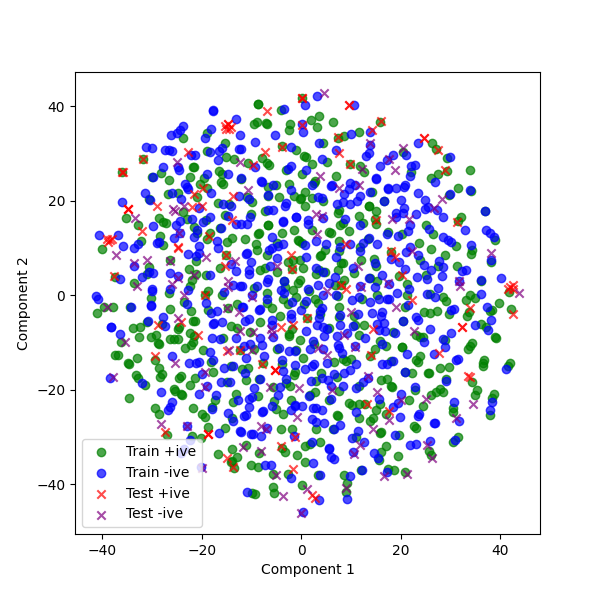
\includegraphics[width=\linewidth]{images/encodings/unsupervised/human/plot_1_1} &
        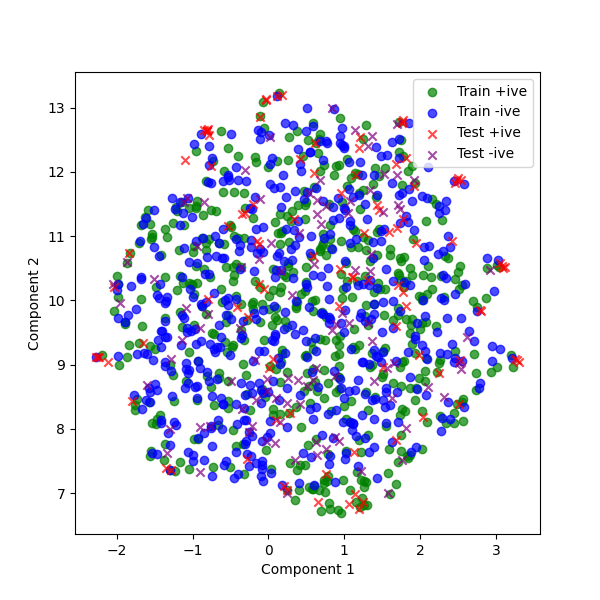
\includegraphics[width=\linewidth]{images/encodings/unsupervised/human/plot_1_2} &
        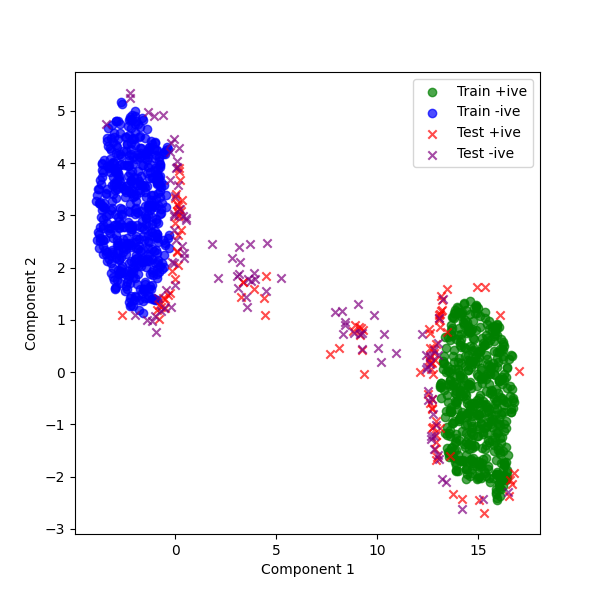
\includegraphics[width=\linewidth]{images/encodings/unsupervised/human/plot_1_3} \\
        \hline
      \end{tabularx}
      \caption{Comparison of all the encodings on human species}\label{tab:dea-unsupervised-encodings-H}
    \end{table}

    \begin{table}[htbp]
      \centering
      \begin{tabularx}{\textwidth}{|p{1cm}|X|X|X|}
        \hline
        &
        tSNE &
        UMAP &
        UMAP (fitted) \\
        \hline
        \rotatebox{90}{\parbox{4cm}{\centering Binary}} &
        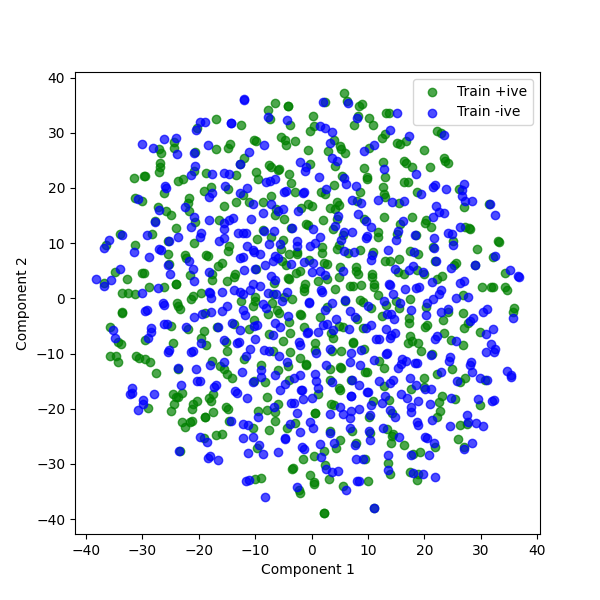
\includegraphics[width=\linewidth]{images/encodings/unsupervised/mouse/plot_1_1} &
        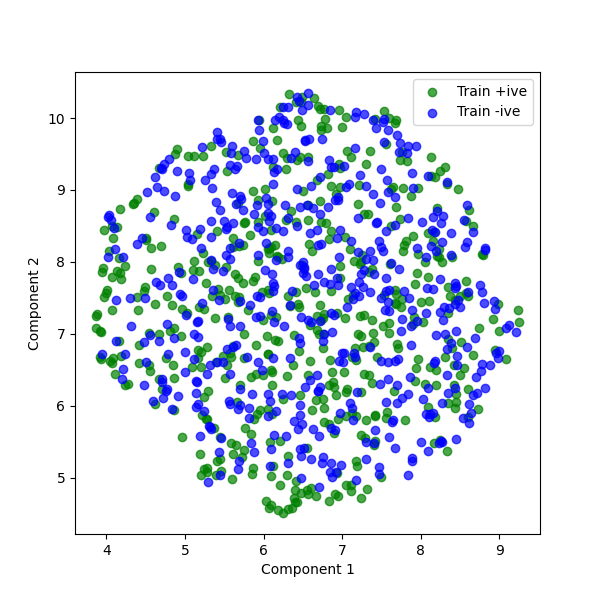
\includegraphics[width=\linewidth]{images/encodings/unsupervised/mouse/plot_1_2} &
        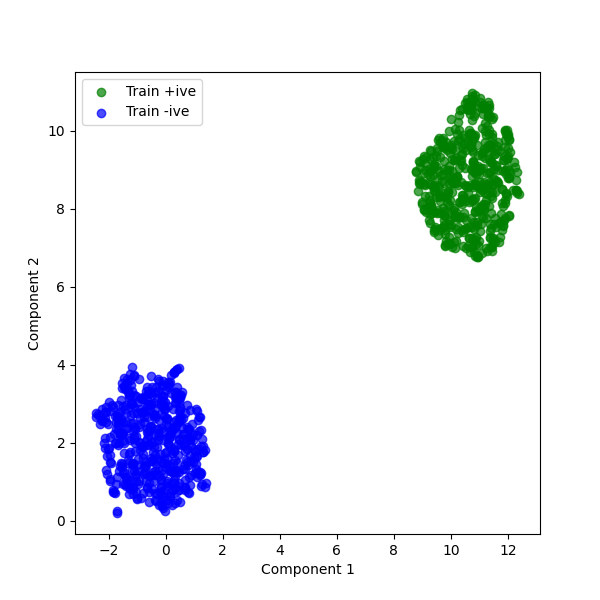
\includegraphics[width=\linewidth]{images/encodings/unsupervised/mouse/plot_1_3} \\
        \hline
      \end{tabularx}
      \caption{Comparison of all the encodings on mouse species}\label{tab:dea-unsupervised-encodings-M}
    \end{table}

    \begin{table}[htbp]
      \centering
      \begin{tabularx}{\textwidth}{|p{1cm}|X|X|X|}
        \hline
        &
        tSNE &
        UMAP &
        UMAP (fitted) \\
        \hline
        \rotatebox{90}{\parbox{4cm}{\centering Binary}} &
        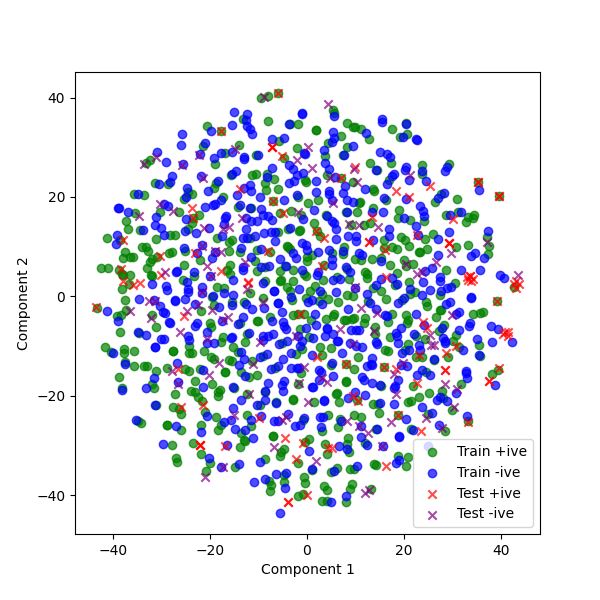
\includegraphics[width=\linewidth]{images/encodings/unsupervised/yeast/plot_1_1} &
        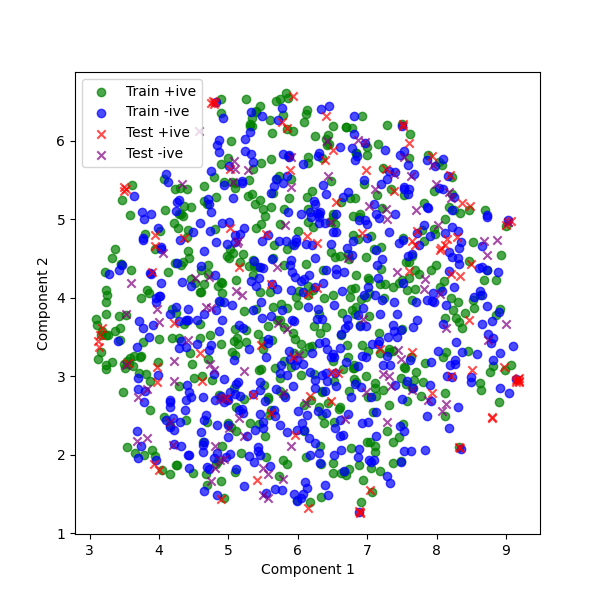
\includegraphics[width=\linewidth]{images/encodings/unsupervised/yeast/plot_1_2} &
        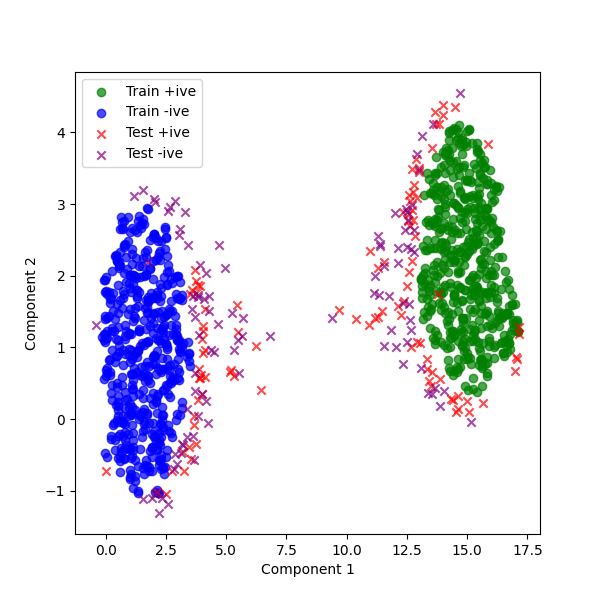
\includegraphics[width=\linewidth]{images/encodings/unsupervised/yeast/plot_1_3} \\
        \hline
      \end{tabularx}
      \caption{Comparison of all the encodings on yeast species}\label{tab:dea-unsupervised-encodings-S}
    \end{table}

    These projections allow us to explore the structure of the data across species and encoding schemes.
    In particular, the supervised UMAP provides insights into how well the encoded features separate the data according to the target labels, which is crucial for understanding the effectiveness of the encoding in downstream predictive tasks.

    But based on the information that we see in the visualizations, we can clearly see that there is no significant correlation between data since in all cases the data is highly overlapping regardless of the encoding used, the first two columns show the usage of tSNE and UMAP adn they are just used for dimensionality reduction however in the 3rd column we use UMAP but we fit it on the training set, then we analyse the relationship between trest and training set and we notice that even after training the data there is no correlation between the positive-positive of training and testing set and negative-negative of training and testing set which makes the classification problem very challenging, in the next section we will analyse some errors in the exiting studies and will re-evaluate the results, since our current observation states that the classification with high accuracy is not possible because of absense of correlation in data.

%    in the next section we try to apply different distance algorithms on the samples to check their relationships and see if the classification boundary exists or not.
